\section{Networks}
There are several terms in the network domain, and this section will contain descriptions of networks and network theory, as well as definitions used in this report. 

The implementation of a communication network is necessary, as the sensor system is supposed to reduce the amount of work for measuring the soil properties on the golf course. The current method of measurement is time-consuming, because of the travel time used to cover the designated area of the golf course. A network implementation of the sensor system can transmit the data gathered from each sensor to an end point.

A computer network is a collection of computers and devices connected so that they can share information and services \cite{mansfield2009computer}. Devices and connections in computer networks can be modeled with graphs, and therefore the network terminology used will be similar to graph terminology. 

%The communication structure the devices use to exchange information over a medium is called protocol, which will be described in another section.

%Definitions:
% Node: device in the network
% Edge: connection in the network
% Topology: arrangement/structure of objects
% Destination node: main node/gateway/ {[raspberry 3.14]}
% Gateway
% Relay
% Routing
% Flooding
% Data: transmitted information

A topology is any arrangement of nodes that can be connected with edges \cite[p.~628]{discMath}. A network topology is the arrangement of the nodes, using edges as the structure. There are different types of network topologies and following are some examples:
\begin{itemize}
	\item Ring
	\item Tree
	\item Star
	\item Mesh
\end{itemize}

Examples of these can be seen in figure \ref{fig:topologies}.

\begin{figure}[h!]
	\centering
	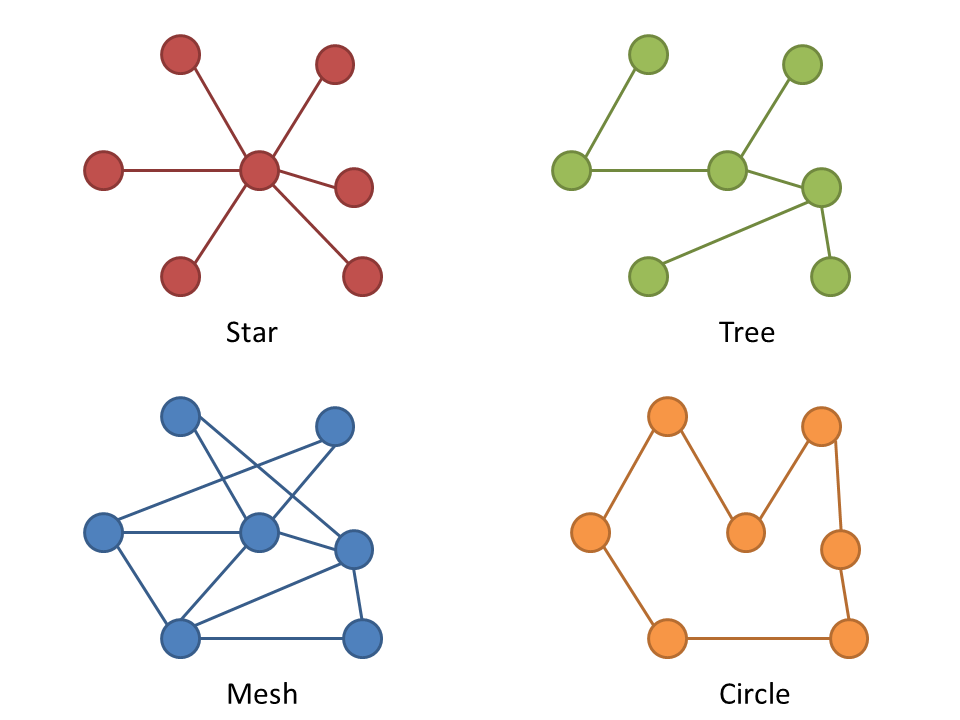
\includegraphics[width=0.8\textwidth]{figures/topologies.png}
	\caption{Network topologies.}
	\label{fig:topologies}
\end{figure}

The star topology, seen in figure \ref{fig:topologies}, has one main node that the other nodes are directly connected to. An example of a star topology network is Wi-Fi, typically with a wireless router to which other devices are connected to gain network access. The wireless router will handle the network communication and redirect the information to the correct device. A limitation of the star network is that all nodes must have a direct connection to the main node, and should therefore be within transmitting range of the main node.

A tree topology, seen in figure \ref{fig:topologies}, utilizes a main node, called the root of the tree. The devices in the network do not necessarily connect directly to the main node, but rather connect to another node that relays to the main node. This can repeat over multiple levels, so that information is relayed through several nodes, before reaching the main node. The tree network has a fixed node structure, and the nodes will relay and route the information towards the destination \cite{kizza2015guide}. It has a reach advantage over the star topology, as data of nodes, not directly within reach of the main node, can still be delivered to the destination node.

The ring topology, seen in figure \ref{fig:topologies}, connects all nodes in a circuit where the path passes through all nodes exactly once. This topology does not require a central node to control the data communication, and will, like the tree topology, relay the data through a certain chain of nodes before it reaches the destination node. It is vulnerable, while there is only two directions to communicate, and if a connection is lost, there could be a block in the data flow since the data must be sent through all nodes to get to the destination. If any edge is removed from the circuit, the remaining graph is a line, resulting in a chain of communication.

% It is a type of mobile ad hoc network.
Another topology is the mesh, also in figure \ref{fig:topologies}. There are two kinds of mesh networks: The full-mesh and the partial-mesh networks. A full-mesh describes a network where all the nodes are interconnected, similar to a fully connected graph. In this topology, there will be no redirecting or relaying, but just a direct connection to the destination node, regardless of the destination. A partial mesh is also a mesh network, but does not require all nodes to be connected, so that it's similar to a tree topology, but cycles can occur. The partial-mesh must then support relaying of data, to transfer data from any node to the destination node.

A summary of the network topology strength and weaknesses is show in table \ref{tab:topologies}.
\begin{figure}
\begin{adjustwidth}{-1.5cm}{}
\rowcolors{2}{gray!25}{gray!7}
\def\arraystretch{1.1}
	\begin{tabular}{lll}
		Topology & Pros    & Cons \\ 
		\hline
		Ring     & Limited to two directions of communication                                                                               & \begin{tabular}[t]{@{}l@{}}Requires some ring formation\\ of the nodes in the network\\ Information delay through the network\end{tabular} \\
		Tree     & \begin{tabular}[t]{@{}l@{}}Reach through internode communication\\ from leaves to root\end{tabular}                                                                 & \begin{tabular}[t]{@{}l@{}}Cannot contain loops\end{tabular}                                                                                                                     \\
		Star     & Fast, direct communication to main node                                                                                  & \begin{tabular}[t]{@{}l@{}}All nodes must have transmit reach\\ covering the main node\end{tabular}                                                                                \\
		Mesh     & \begin{tabular}[t]{@{}l@{}}Reach through internode communication\\ Not critically sensitive to node failure\end{tabular} & Information delay through the network                                                                                                   
	\end{tabular}
	\caption{Topology strengths and weaknesses.}
	\label{tab:topologies}
	\end{adjustwidth}
\end{figure}%The mesh networks have the same limitation as a tree network, regarding the information transmission delay because the information transmits through up to several nodes. \cite{g2wmn}

%The best fitting network topology for the use case is a mesh network. It can transmit information through the network without limiting the connected devices to a certain distance from a main device, as with a star topology. It is also capable of multiple methods of distributing information. It does not rely on all nodes working at all times, as the network can reconfigure and find another path of information. This applies as long as there somehow exists another node that can relay the information towards the main node.

%\todo{Move this paragraph to protocols?}
%There are multiple methods of communicating through a mesh network, therein routing and flooding are two alternatives. Routing will transfer the information to the destination node through a determined route, whereas the flooding method will notify all nodes within reach to distribute the information forward, and this will repeat until all nodes has transmitted the information, and hence the destination node also has received the information.

%''\textit{An ad-hoc wireless network is a wireless network, comprised of mobile computing devices that use wireless transmission for communication, having no fixed infrastructure}'' - \cite{murthy2004ad}. 
